\documentclass[margin=2mm]{standalone}
\usepackage{tikz}
\usepackage{amsmath,amssymb,mathtools}
\begin{document}
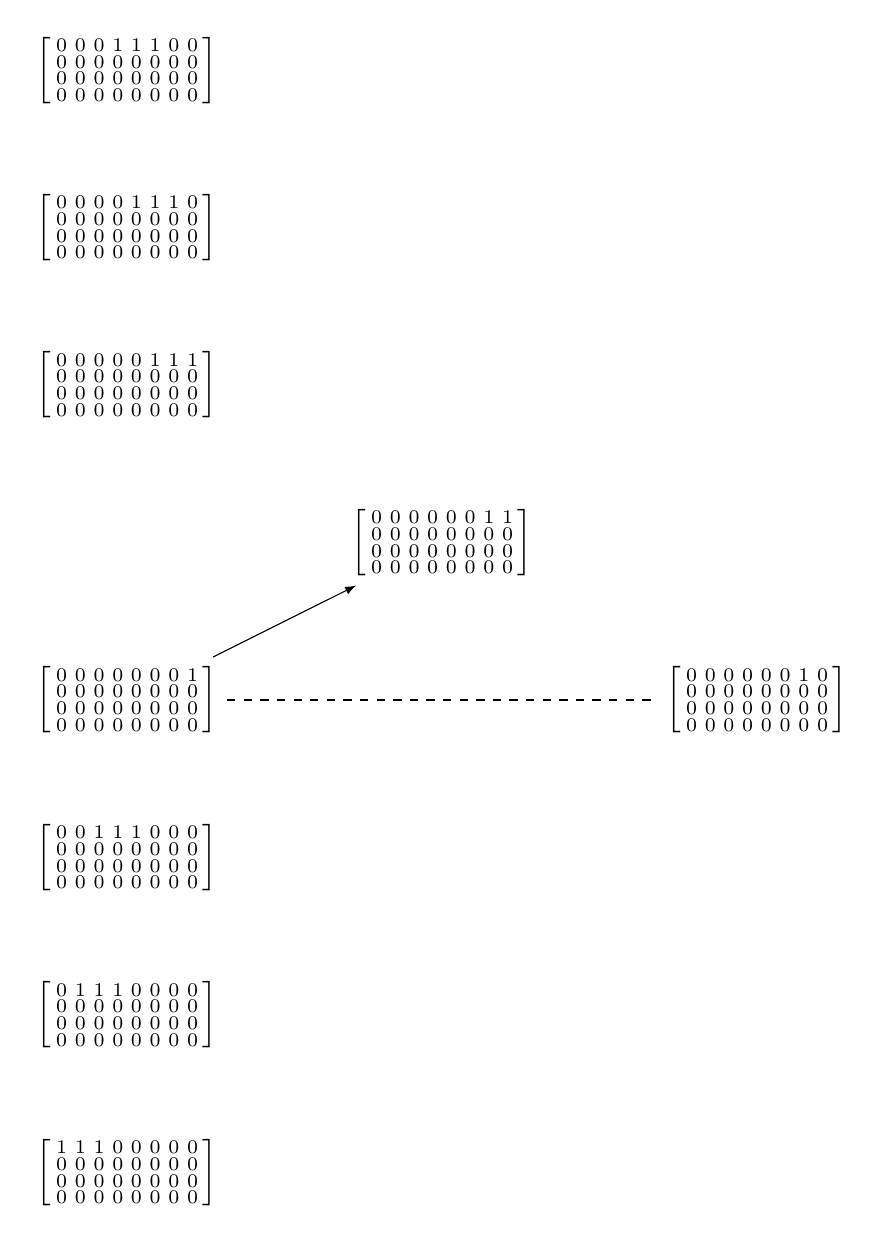
\begin{tikzpicture}[xscale=4,yscale=2]
\node (t-0P0) at (0,-3) [scale=1] {$\begin{bsmallmatrix}
 1 & 1 & 1 & 0 & 0 & 0 & 0 & 0\\
 0 & 0 & 0 & 0 & 0 & 0 & 0 & 0\\
 0 & 0 & 0 & 0 & 0 & 0 & 0 & 0\\
 0 & 0 & 0 & 0 & 0 & 0 & 0 & 0\\
\end{bsmallmatrix}$};
\node (t-0P1) at (0,-2) [scale=1] {$\begin{bsmallmatrix}
 0 & 1 & 1 & 1 & 0 & 0 & 0 & 0\\
 0 & 0 & 0 & 0 & 0 & 0 & 0 & 0\\
 0 & 0 & 0 & 0 & 0 & 0 & 0 & 0\\
 0 & 0 & 0 & 0 & 0 & 0 & 0 & 0\\
\end{bsmallmatrix}$};
\node (t-0P2) at (0,-1) [scale=1] {$\begin{bsmallmatrix}
 0 & 0 & 1 & 1 & 1 & 0 & 0 & 0\\
 0 & 0 & 0 & 0 & 0 & 0 & 0 & 0\\
 0 & 0 & 0 & 0 & 0 & 0 & 0 & 0\\
 0 & 0 & 0 & 0 & 0 & 0 & 0 & 0\\
\end{bsmallmatrix}$};
\node (t-0P3) at (0,4) [scale=1] {$\begin{bsmallmatrix}
 0 & 0 & 0 & 1 & 1 & 1 & 0 & 0\\
 0 & 0 & 0 & 0 & 0 & 0 & 0 & 0\\
 0 & 0 & 0 & 0 & 0 & 0 & 0 & 0\\
 0 & 0 & 0 & 0 & 0 & 0 & 0 & 0\\
\end{bsmallmatrix}$};
\node (t-0P4) at (0,3) [scale=1] {$\begin{bsmallmatrix}
 0 & 0 & 0 & 0 & 1 & 1 & 1 & 0\\
 0 & 0 & 0 & 0 & 0 & 0 & 0 & 0\\
 0 & 0 & 0 & 0 & 0 & 0 & 0 & 0\\
 0 & 0 & 0 & 0 & 0 & 0 & 0 & 0\\
\end{bsmallmatrix}$};
\node (t-0P5) at (0,2) [scale=1] {$\begin{bsmallmatrix}
 0 & 0 & 0 & 0 & 0 & 1 & 1 & 1\\
 0 & 0 & 0 & 0 & 0 & 0 & 0 & 0\\
 0 & 0 & 0 & 0 & 0 & 0 & 0 & 0\\
 0 & 0 & 0 & 0 & 0 & 0 & 0 & 0\\
\end{bsmallmatrix}$};
\node (t-0P6) at (1,1) [scale=1] {$\begin{bsmallmatrix}
 0 & 0 & 0 & 0 & 0 & 0 & 1 & 1\\
 0 & 0 & 0 & 0 & 0 & 0 & 0 & 0\\
 0 & 0 & 0 & 0 & 0 & 0 & 0 & 0\\
 0 & 0 & 0 & 0 & 0 & 0 & 0 & 0\\
\end{bsmallmatrix}$};
\node (t-0P7) at (0,0) [scale=1] {$\begin{bsmallmatrix}
 0 & 0 & 0 & 0 & 0 & 0 & 0 & 1\\
 0 & 0 & 0 & 0 & 0 & 0 & 0 & 0\\
 0 & 0 & 0 & 0 & 0 & 0 & 0 & 0\\
 0 & 0 & 0 & 0 & 0 & 0 & 0 & 0\\
\end{bsmallmatrix}$};
\node (t-1P7) at (2,0) [scale=1] {$\begin{bsmallmatrix}
 0 & 0 & 0 & 0 & 0 & 0 & 1 & 0\\
 0 & 0 & 0 & 0 & 0 & 0 & 0 & 0\\
 0 & 0 & 0 & 0 & 0 & 0 & 0 & 0\\
 0 & 0 & 0 & 0 & 0 & 0 & 0 & 0\\
\end{bsmallmatrix}$};
\draw[-latex] (t-0P7) -- (t-0P6);
\draw[dashed] (t-0P7)--(t-1P7);
\end{tikzpicture}\end{document}